\subsection{Fluid Systems}

There are many considerations when it comes to the design of the feed system for a small-scale air-breathing rotating detonation engine. The goals of project SABR are to design, build and test the RDE and determine the ranges of total mass flow rate and equivalence ratios over which the RDE can operate and produce stable detonation. This section will introduce and cover propellant feed systems in the context of the project as well as the fundamental principles of fluidic hardware, fluid flow, and the safety and handling of high-pressure systems.

Small size RDEs reduce the requirements for fuel and oxidizer flow rates, which makes the RDE more portable and easier to iterate upon \cite{dechert:2020}. This is due to the fact that small-scale RDEs have small channel geometries, which inherently results in lower mass flow rates and higher frequencies of operation \cite{dechert:2020, fiorino:2021, fiorino:2022}. One of the biggest challenges will be refreshing propellants at a high enough rate into the chamber with enough time and energy for proper reactant mixing. This will mainly fall under the responsibility of the injector. However, it will help to have a precise, steady, and repeatable feed of propellants into the injector plenums to help reduce transience in the system. Flow rates are acquired through relations between detonation cell size, chamber radii, channel widths, combustor lengths, and operational frequencies. Equivalence ratios are a result of chemical equilibrium considerations and will be calculated to maximize the reaction efficiency. \cite{yokoo:2019}. Given an equivalence ratio and associated propellant mass flow rates, as well as desired plenum pressures the feed system becomes simplified, focusing solely on providing and recording the mass flow rates and pressures with high accuracy and consistency.

\begin{figure}[ht]
    \centering
    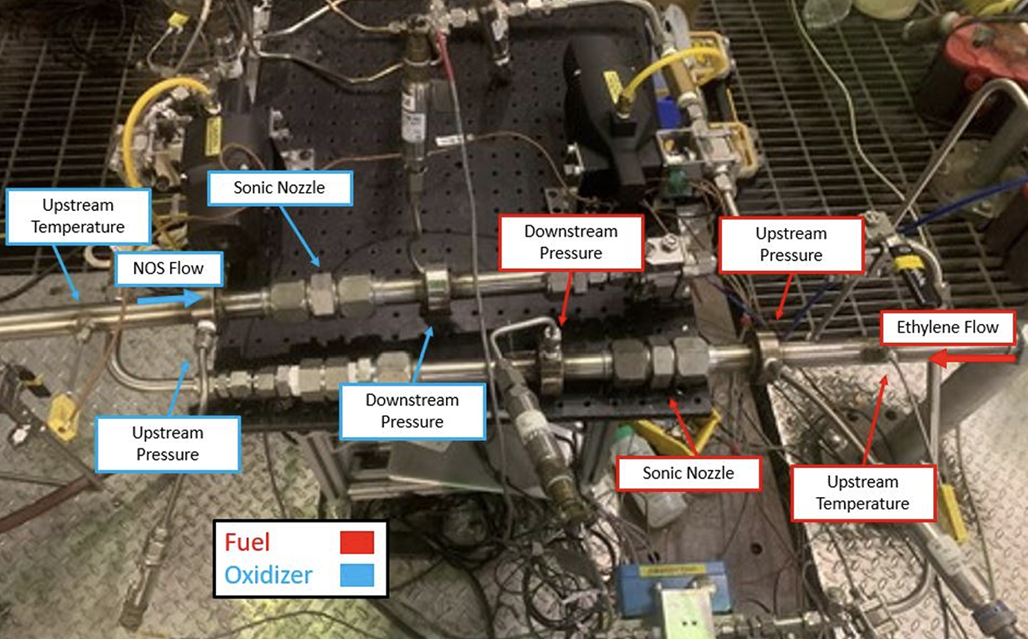
\includegraphics[width=0.75\linewidth]{rde_feed_system_example.png}
    \caption{Example of an RDE feed system (from Wyatt)}
    \label{fig:rde-feed-system-example}
\end{figure}

As mentioned before, one of the primary difficulties with feed systems for small scale RDEs is that the reactants must be supplied into the detonation channel at a rate fast enough so that they are refreshed prior to each passing wave \cite{dechert:2020, fiorino:2021, fiorino:2022}. The amount of time available to refresh the reactants can be extremely short in RDEs. It is even shorter when you consider that the detonation wave passing over the injector inlets can temporarily block the flow of fuel and oxidizer through the injector into the detonation channel due to its extreme pressures \cite{dechert:2020}. The total mass flow rate that of propellants that needs to be provided to the engine will come from the engine specifications. Required mass flow rates of propellants for the detonation reaction has dependence on cell size, fill height, channel length, and channel gap \cite{dechert:2020, fiorino:2021, connolly-boutin:2021, bykovskii:2012}. To determine the detonation frequency for a given RDE, the detonation velocity must be known. Detonation velocity can be a function of many factors to include fuel/oxidizer type and equivalence ratio \cite{dechert:2020, bykovskii:2012}. The detonation cell size is important since the necessary height of the fresh propellants for sustained detonation is directly related to the cell size \cite{bykovskii:2012, russo:2011}.

Changes in mass flow rates have been found to have significant effects on the detonation reaction, especially on the number of waves \cite{law:2021}. At low mass flows create fewer wave detonation at lower frequencies \cite{fiorino:2022, law:2021}. Equivalence ratio and mass flow rates will be calculated using isentropic flow equations and mass flow rate equations such as shown in Figure 2 \cite{nasa-mass-flow-choking:2021, nasa-mass-flow-equations:2021}. Conditions will be calculated upstream using reservoir conditions and readings from pressure gauges. Flow restrictions such as regulators and orifices will be used to control flow rates.

In prior testing with RDEs it has been shown that mass flow instruments have a difficult time accurately measuring mass flow rates due to the pressure oscillations and transient conditions of the flow. It has been shown that sonic orifices can be used to successfully measure mass flow rates by choking the flow at the orifice. Using upstream conditions and the dimensions of the orifice, a mass flow rate can be calculated. When this flow rate is time averaged over the length of the test, it has been shown to produce accurate measurements.

To simulate air-breathing conditions, three feed lines will be used. O$_2$ and GN$_2$ lines will be mixed upstream of the injector to simulate different oxidizer dilutions, with the ultimate goal being a 79\% dilution of the oxygen to simulate air as the oxidizer. All three lines will be similar in setup, using sonic orifices to control and measure mass flow rates. There will also be other lines extending off of the propellant lines which will be used to feed the pre-detonation/ignition system. Plenums allow for the fuel and oxidizer to be distributed to the injector holes of the injector plate. Plenum to chamber pressure ratios determine chocked flow conditions at the injector and can influence the characteristics of the detonation \cite{fiorino:2022, yokoo:2019}. Flow will be sonic at the injector holes because the pressure difference will be controlled to be large enough to meet sonic conditions.

Choking is typically assumed at the injectors. However, the propagation of the detonation wave creates regions of high pressure downstream which could temporarily disturb the choking conditions causing pressures in the line to increase to sustain mass flow rates into the chamber \cite{yokoo:2019}. Otherwise, if the injector is choked, plenum pressures should remain constant. As the detonation wave passes over the injector holes, the high pressure can force products back into the fuel/oxidizer plenum which would have adverse effects on the equivalence ratio and the stability of the detonation wave \cite{dechert:2020}. Therefore, it is critical that choking conditions are achieved at the injector inlet and that the pressures in the plenum allow for this.

The flow of oxidizer and fuel will require flow control devices and a precise control system. Valves of different types will be considered and implemented to reach these requirements. To have precise and repeatable control, solenoid valves will be controlled with DAQ hardware and a driving software to send valve actuation signals. The test setup will also record flow, pressure, temperature, and thrust data.

Understanding the effects of friction on fluid flow through the piping system will be crucial for optimal performance. Parameters such as the coefficient of discharge area (C$_d$A) or flow coefficient (C$_v$) will be used to characterize pressure drops across flow restrictions such as bends in tubing, valves, and orifices \cite{crane-co:1982, asme-fluid-flow:2004, nasa-tubing:2019}. Bends and fittings in the tubing, rough inner surfaces, and restrictions from valves will contribute to energy losses in the system. It will be essential to design and model the flow paths to ensure proper pressures and mass flow rates throughout the system.

Several different types of fluidic connections will likely be used in the system. These could include compression, such as Swagelok, ORB (O-ring boss), NPT (National Pipe Thread), cone-and-thread, and flared fittings (such as JIC 37-degree). Due to the high-pressure applications in this system, Swagelok and NPT fittings are the most likely to be used, as they have some of the best sealing abilities under extreme conditions. The system will incorporate stainless steel tubing of varying thickness to accommodate the different pressure ranges and flow rates that will be required. These parameters will need to be balanced carefully to minimize pressure drops across the system, ensure proper seals, and optimize the safety and performance of the engine.

During the testing phase, the team will be handling high-pressure fluids, including oxidizers like oxygen (O$_2$), fuels such as hydrogen (H$_2$) and inert gases such as gaseous nitrogen (GN$_2$). Given the hazardous nature of these fluids, strict precautions will be implemented during storage and interactions. Oxygen, as an oxidizer, increases the risk of combustion in the presence of flammable materials, necessitating specialized handling procedures and oxygen-safe environments. Inert gases like GN$_2$, while non-flammable, will still be managed under high-pressure conditions, requiring careful attention to equipment and safety protocols to prevent leaks or failures. All personnel will follow rigorous safety guidelines, including personal protective equipment (PPE) use, continuous monitoring of pressure levels, and adherence to standardized handling procedures for high-pressure gases \cite{aiga-hydrogen-supply:2024, aiga-oxygen-cleaning:2019, nasa-oxygen-systems:1996}.

This project will involve managing extremely high temperatures and pressures, especially when dealing with the detonation reaction. The system will also have potentially hazardous combustion products, including gases containing fine particulate matter. The team must utilize proper pressure fittings that are compatible with these fluids and rated for these conditions to minimize the risk of leaks, failures, and contamination from foreign object debris (FOD). The presence of small solid particles and other material poses a significant risk for contaminating the system, especially considering the very small areas at which flows will be choked or reach sonic conditions. These contaminants can cause pressure buildups, reduce flow rates, and damage components, all of which could cause catastrophic failure of the system. To mitigate these risks, the team will implement proper cleaning procedures, particularly oxygen cleaning, to ensure oxidizer-safe environments and prevent clogging or build-up of material in the flow paths \cite{aiga-oxygen-cleaning:2019}. Maintaining clean lines will be essential for both the team’s safety and the engine's health.

Managing high pressures is a fundamental aspect of this system's design. Over-pressurization presents a severe risk to both the system and personnel. Therefore, pressure relief valves (PRVs) and burst discs will be incorporated into the fluid system to provide a fail-safe for excessive pressure buildup. PRVs will open automatically to release pressure when it exceeds safe limits and burst discs will rupture at a specific pressure threshold, providing an emergency pressure release mechanism. The feed system will be designed to have pressure relief lines to prevent trapped pressure, and valves will be selected to ensure that they fail into “safe” positions in the event of power losses. Pressure relieving components and careful system design are critical for ensuring the safety of the system and of operators during hazardous operations. 

In conclusion, designing the feed system for a small-scale air-breathing rotating detonation engine involves several significant challenges. The engine’s reliance on pressure gain combustion means precise control of mass flow rates, equivalence ratios, and reactant mixing is critical. These challenges are amplified in small-scale systems, where limited space and rapid refresh rates make achieving stable detonation more difficult. Careful consideration of fluid dynamics, appropriate hardware, and safety measures will be essential to ensure the engine operates efficiently and safely in these extreme conditions.

The success of this project depends on developing a robust feed system that can handle high pressures and temperatures while preventing the backflow of detonation products. Selecting the right fittings, flow control valves, and pressure management tools will be crucial for maintaining safe and stable operation. Additionally, special attention to factors such as friction, contaminants, and pressure drops will help ensure consistent fuel and oxidizer flow, optimizing engine performance. This approach will provide the necessary groundwork for designing, building, and testing an RDE capable of stable detonation under a variety of conditions, advancing the understanding and development of pressure gain combustion technologies.